% Options for packages loaded elsewhere
\PassOptionsToPackage{unicode}{hyperref}
\PassOptionsToPackage{hyphens}{url}
%
\documentclass[
]{article}
\usepackage{amsmath,amssymb}
\usepackage{lmodern}
\usepackage{iftex}
\ifPDFTeX
  \usepackage[T1]{fontenc}
  \usepackage[utf8]{inputenc}
  \usepackage{textcomp} % provide euro and other symbols
\else % if luatex or xetex
  \usepackage{unicode-math}
  \defaultfontfeatures{Scale=MatchLowercase}
  \defaultfontfeatures[\rmfamily]{Ligatures=TeX,Scale=1}
\fi
% Use upquote if available, for straight quotes in verbatim environments
\IfFileExists{upquote.sty}{\usepackage{upquote}}{}
\IfFileExists{microtype.sty}{% use microtype if available
  \usepackage[]{microtype}
  \UseMicrotypeSet[protrusion]{basicmath} % disable protrusion for tt fonts
}{}
\makeatletter
\@ifundefined{KOMAClassName}{% if non-KOMA class
  \IfFileExists{parskip.sty}{%
    \usepackage{parskip}
  }{% else
    \setlength{\parindent}{0pt}
    \setlength{\parskip}{6pt plus 2pt minus 1pt}}
}{% if KOMA class
  \KOMAoptions{parskip=half}}
\makeatother
\usepackage{xcolor}
\usepackage{graphicx}
\makeatletter
\def\maxwidth{\ifdim\Gin@nat@width>\linewidth\linewidth\else\Gin@nat@width\fi}
\def\maxheight{\ifdim\Gin@nat@height>\textheight\textheight\else\Gin@nat@height\fi}
\makeatother
% Scale images if necessary, so that they will not overflow the page
% margins by default, and it is still possible to overwrite the defaults
% using explicit options in \includegraphics[width, height, ...]{}
\setkeys{Gin}{width=\maxwidth,height=\maxheight,keepaspectratio}
% Set default figure placement to htbp
\makeatletter
\def\fps@figure{htbp}
\makeatother
\setlength{\emergencystretch}{3em} % prevent overfull lines
\providecommand{\tightlist}{%
  \setlength{\itemsep}{0pt}\setlength{\parskip}{0pt}}
\setcounter{secnumdepth}{-\maxdimen} % remove section numbering
\ifLuaTeX
  \usepackage{selnolig}  % disable illegal ligatures
\fi
\IfFileExists{bookmark.sty}{\usepackage{bookmark}}{\usepackage{hyperref}}
\IfFileExists{xurl.sty}{\usepackage{xurl}}{} % add URL line breaks if available
\urlstyle{same} % disable monospaced font for URLs
\hypersetup{
  pdftitle={Jazler},
  hidelinks,
  pdfcreator={LaTeX via pandoc}}

\title{Jazler}
\author{}
\date{}

\begin{document}
\maketitle

\hypertarget{mode-selection}{%
\section{Mode Selection}\label{mode-selection}}

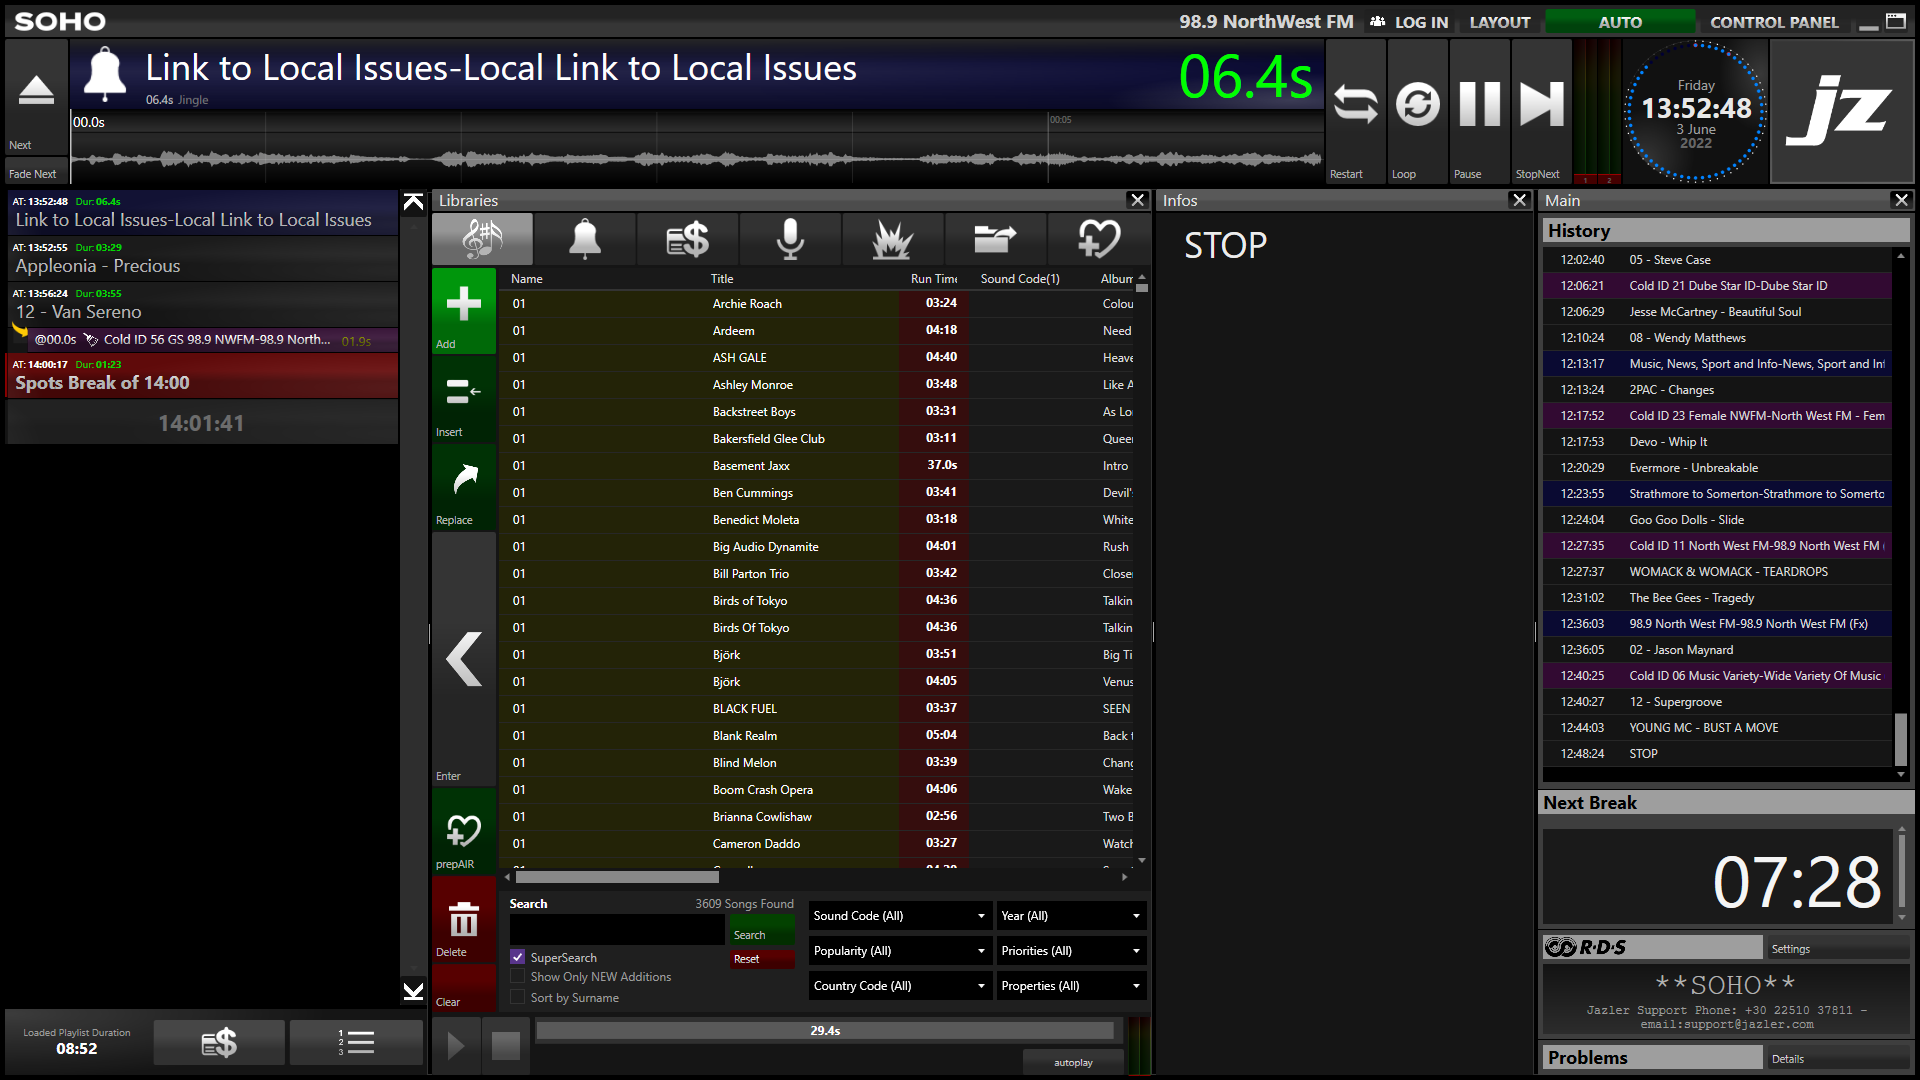
\includegraphics[width=6.26042in,height=3.52083in]{vertopal_03fa0a741e214d36912ab6bc9018a8aa/media/image1.png}

Figure 0‑1 Jazler Main Screen

To change the operation mode of Jazler, click on the mode button found
on the top line of the screen. This button will display the current mode
of jazler (Manual, Auto, Offline)

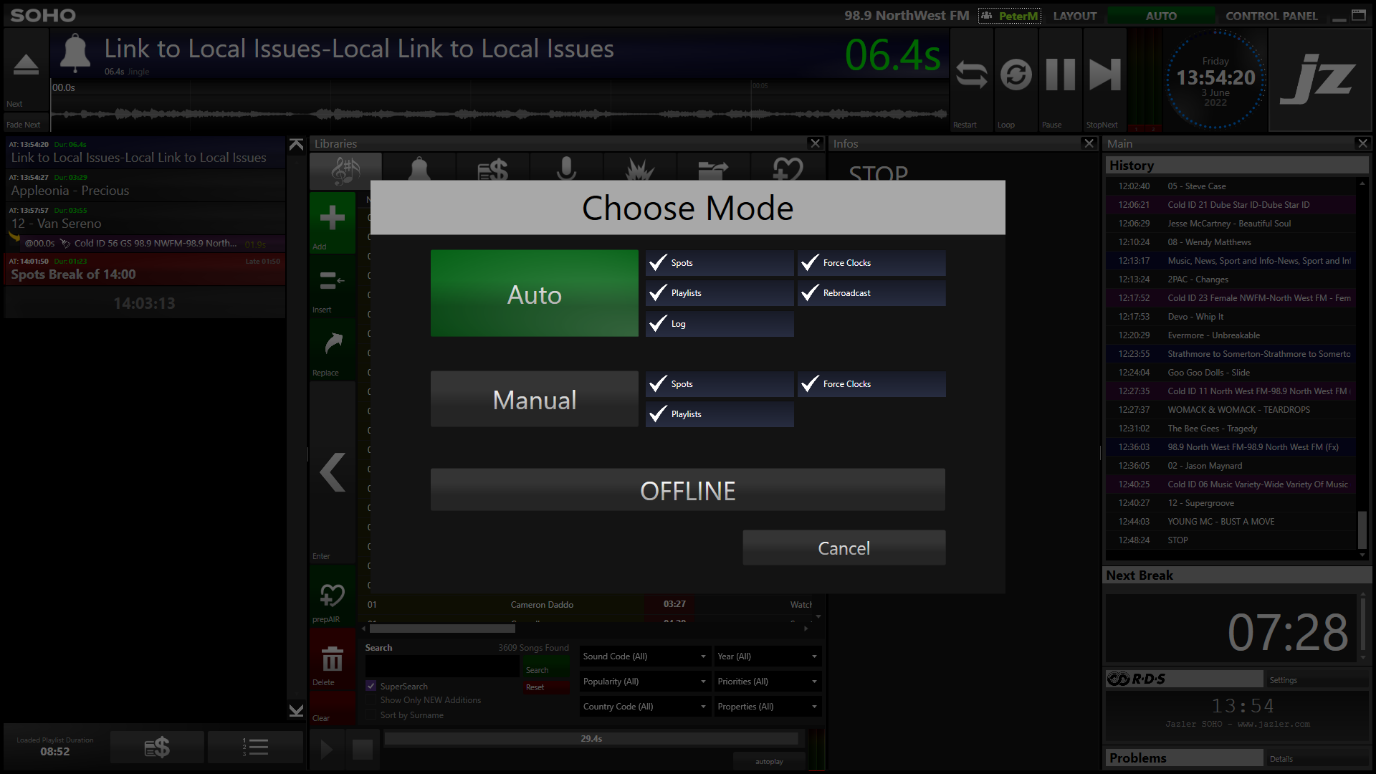
\includegraphics[width=2.85433in,height=1.86944in]{vertopal_03fa0a741e214d36912ab6bc9018a8aa/media/image2.png}Auto
mode is used for when the studio in automation / unattended mode, such
as overnight or when a live presenter in unavailable.

Figure 0‑2 Auto mode button

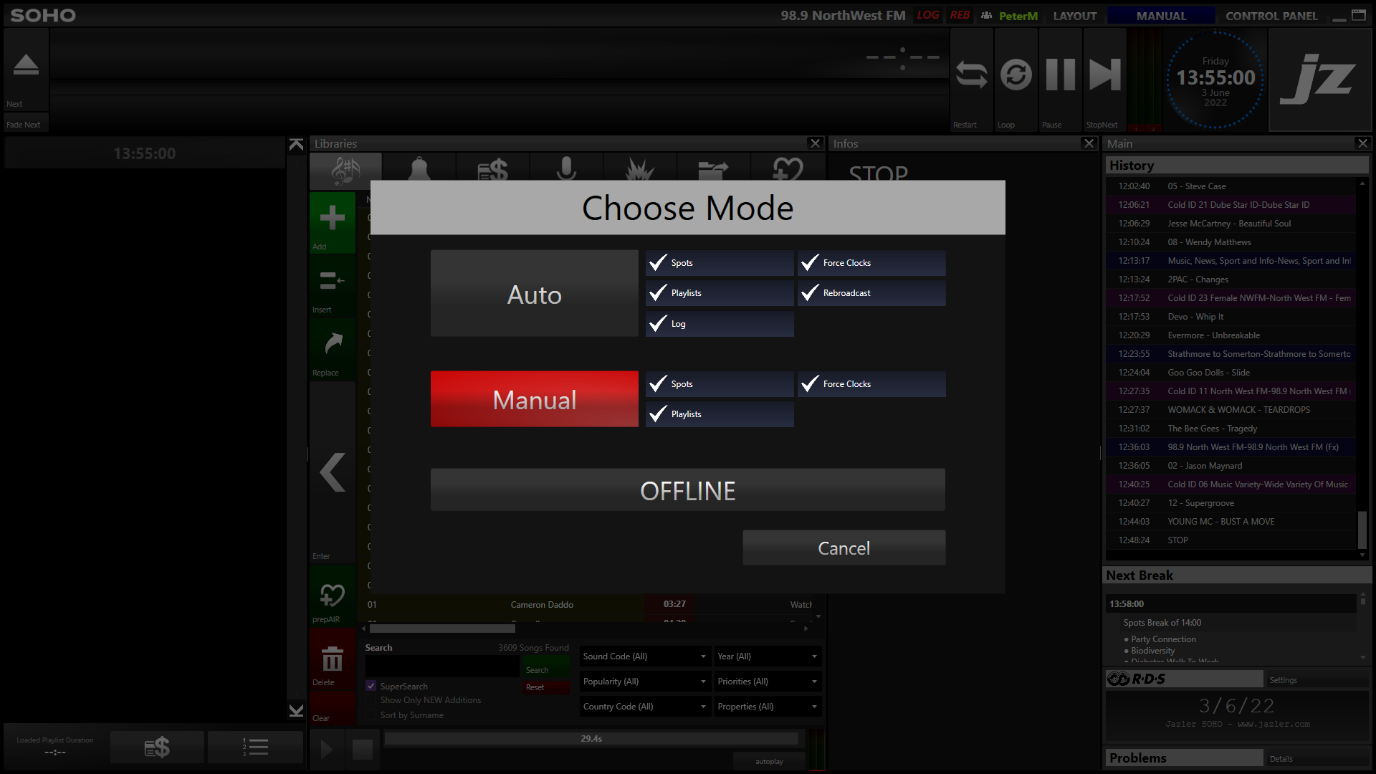
\includegraphics[width=2.85417in,height=1.87008in]{vertopal_03fa0a741e214d36912ab6bc9018a8aa/media/image3.png}Manual
mode is used when a live presenter is present. In this mode, you will be
alerted when a scheduled break is due to play, and then must be played
manually.

Figure 0‑3 Manual mode button

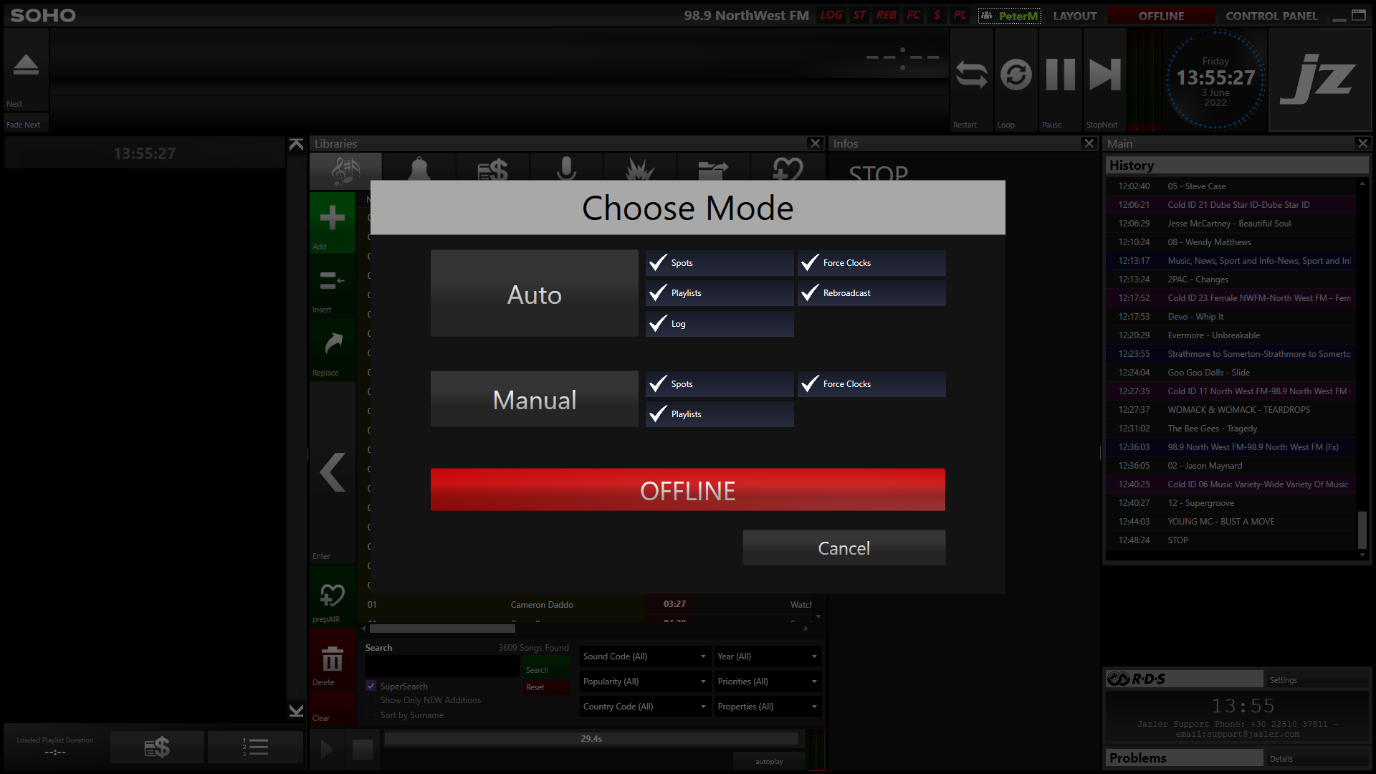
\includegraphics[width=2.85433in,height=1.86944in]{vertopal_03fa0a741e214d36912ab6bc9018a8aa/media/image4.png}Offline
mode is for when a studio is not in use or not on air.

Figure 0‑4 Offline mode button

When you are finished with a studio, and that studio is not being used
by another presenter or automation, please leave it in ``Offline'' mode.

\hypertarget{playing-scheduled-breaks}{%
\section{Playing Scheduled Breaks}\label{playing-scheduled-breaks}}

TODO: How to play scheduled breaks

\end{document}
